%!TEX root = userguide.tex
\section{Downloading and Compiling PEBBL}
\label{sec:downloadcompile}

\subsection{System requirements}
\begin{itemize}
\item A Unix-like operating systems (including Linux, Mac OS X, or some
version of the Linux subsystem for Microsoft Windows).  This guide assumes
basic familiarity with the command-line interface to such environments.
\vspace{-1.8ex}
%% Make below optional if tarballs can be used
\item The \texttt{git} version management system (required for initial download only)
\vspace{-1.8ex}
\item The \texttt{cmake} configuration and build system (including GNU \texttt{make})
\vspace{-1.8ex}
\item A C++ compiler, such as g++
\vspace{-1.8ex}
\item For parallel execution, some form of MPI, such as OpenMPI or MPICH.
\end{itemize}
These packages should be readily installable in most Unix-like
systems.  

The PEBBL distribution also includes some Python scripts, for which a Python
interpreter is needed.  These scripts perform auxiliary functions and are not
required to run PEBBL.


\subsection{Downloading PEBBL}
To download the latest version of PEBBL, issue the following \texttt{git} command:
{\small
\begin{codeblock}
git clone https://github.com/PEBBL/pebbl.git
\end{codeblock}
}
\noindent This command will create a directory called
\texttt{pebbl}.  


\subsection{Structure of the \texttt{pebbl} directory}
\label{sec:dirstruct}
PEBBL's directory structure has been greatly simplified from prior releases.
The subdirectories of \texttt{pebbl} are:
\begin{description}
\item[\texttt{src}]  Contains the source code.  Nearly all the contents of
this directory is within a subdirectory \texttt{pebbl} (which allows PEBBL C++
\texttt{\#include} statements to naturally self documenting).  Within
\texttt{pebbl/src/pebbl}, header and \texttt{.cpp} files are mixed in seven
further directories \texttt{pebbl/src/pebbl/bb} (for ``branch-and-bound''),
\texttt{pebbl/src/pebbl/comm} (for ``communication''), and so forth.
\item[\texttt{data}] Contains data files for the example application programs.
Its subdirectories are \texttt{pebbl/\linebreak[1]data/knapsack} for the
simple knapsack solver and \texttt{pebbl/data/monomial} for the maximum
monomial agreement solver.
\item[\texttt{doc}] Contains documentation, include the PDF of this document.
Currently, the only subdirectory in 
this location is \texttt{pebbl/doc/uguide}, which contains the \LaTeX~source
and other files necessary to produce this document. 
\item[\texttt{scripts}] contains some useful Python scripts related to PEBBL.
\end{description}


\subsection{Configuration}
\label{sec:configure}
PEBBL now uses \texttt{cmake} and an ``out-of-source'' build scheme.  To
configure PEBBL for your system, create another directory at the same level as
the \texttt{pebbl} directory created by \texttt{git}; this directory will hold
your compiled version of PEBBL.  From here on, this document will assume that
this directory is called \texttt{buildpebbl}, but the name can be anything you
wish.

Before compiling, you must configure PEBBL.  To do so, first descend into the
\texttt{buildpebbl} directory.  If you are in an environment with usable X
graphics, then give the command
\begin{codeblock}
cmake-gui ../pebbl
\end{codeblock}
If your system does not have usable X graphics (for example, if running over a
slow remote connection) then instead give the command
\begin{codeblock}
ccmake ../pebbl
\end{codeblock}

\subsubsection{Configuring with \texttt{cmake-gui}}
After you start \texttt{cmake-gui}, a window like the one shown in
Figure~\ref{fig:cmake1} should appear.  Start the configuration process by
pressing the "Configure" button on the lower left, after which a window like
that in Figure~\ref{fig:cmake-choosegen} should pop up.

\begin{figure}[tpb]
\begin{center}
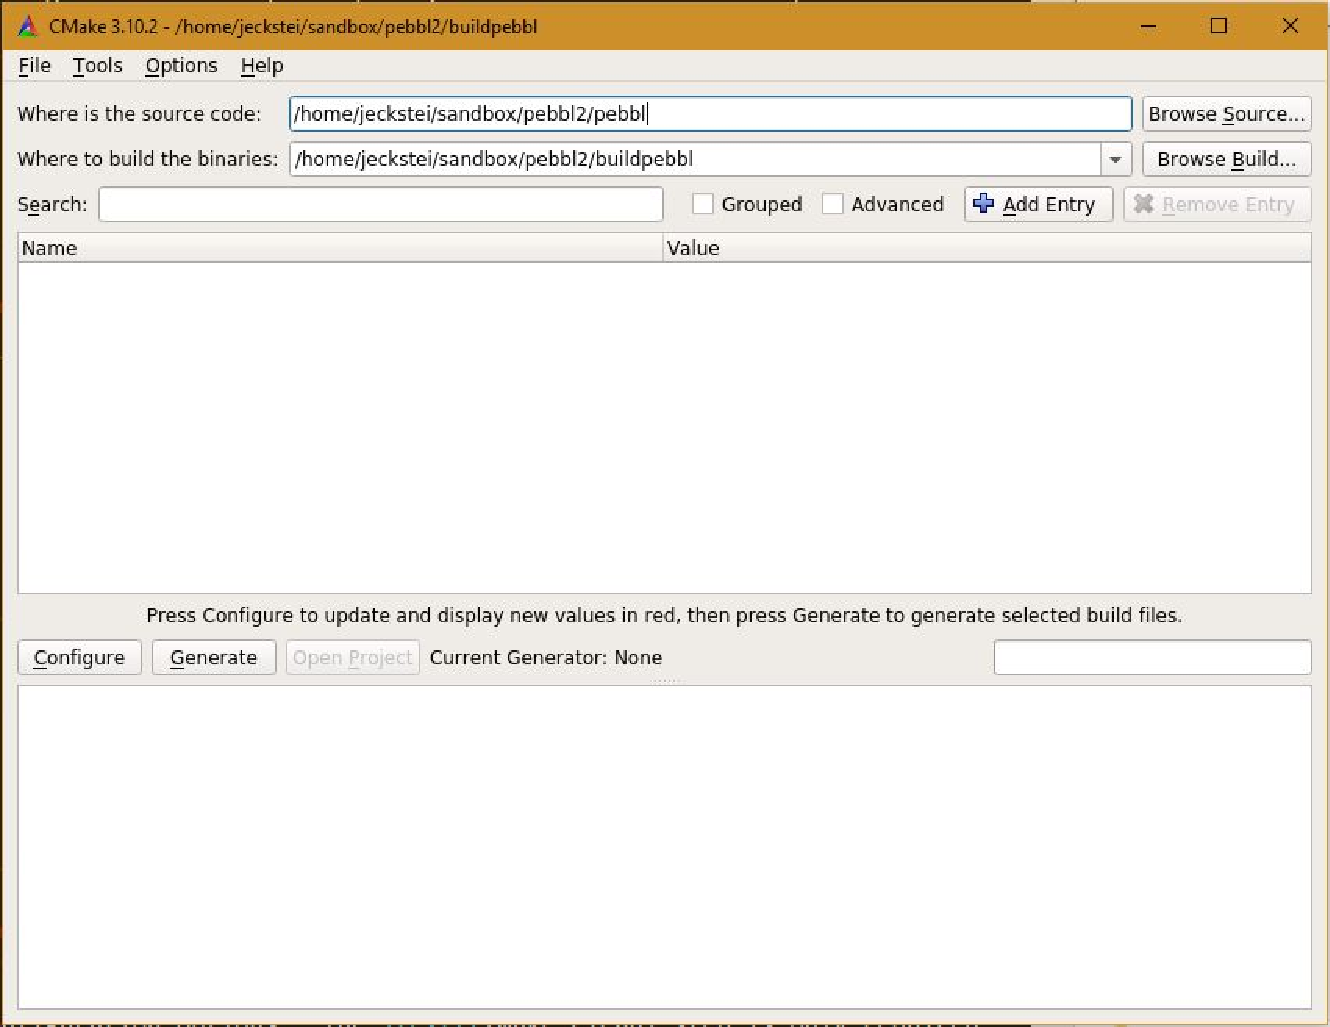
\includegraphics[height=0.45\textheight]{cmake1}
\vspace{-0.3in}
\end{center}
\caption{Initial display from \texttt{cmake-gui}.\label{fig:cmake1}}
\end{figure}

\begin{figure}[tpb]
\begin{center}
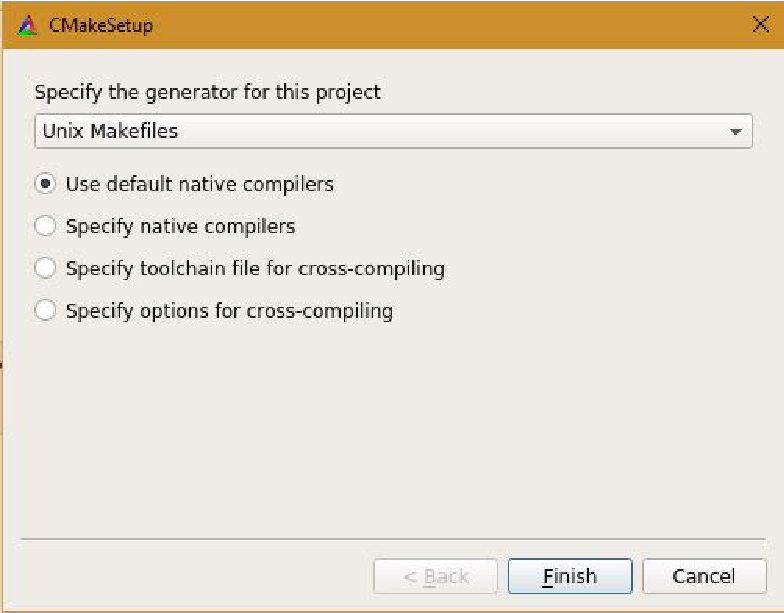
\includegraphics[width=0.45\textwidth]{cmake-choosegen}
\vspace{-0.3in}
\end{center}
\caption{Generator choice pop-up from \texttt{cmake-gui}.\label{fig:cmake-choosegen}}
\end{figure}

For ordinary applications, it is sufficient to press the ``Finish'' button in
this pop-up window, which selects the default native compilers.  If you wish
to specify a non-default C++ compiler or use a cross-configuration
environment, you may select one of the other options.  This guide covers only
the default native case.

The next display from \texttt{cmake-gui} should resemble
Figure~\ref{fig:cmake2}.  You should now select the build options you desire
by modifying the entries in the "Value" column of this display.

\begin{figure}[tpb]
\begin{center}
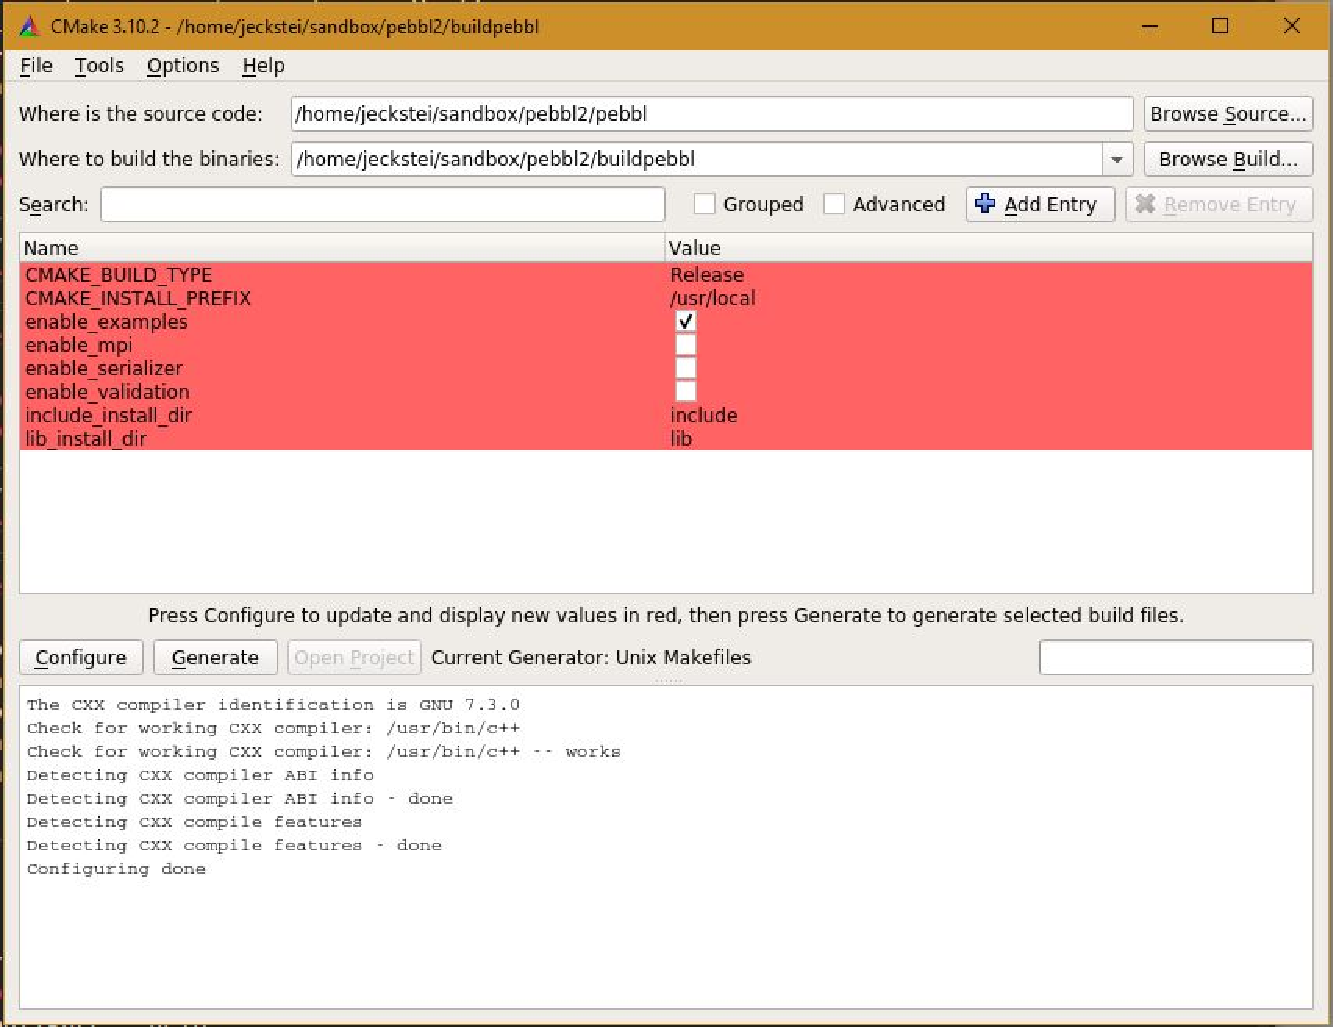
\includegraphics[height=0.45\textheight]{cmake2}
\vspace{-0.3in}
\end{center}{}
\caption{Appearance of \texttt{cmake-gui} after initial configuration step.
  \label{fig:cmake2}}
\end{figure}

\begin{description}
\item[\texttt{CMAKE\_BUILD\_TYPE}:] The default value ``Release'' builds a
version of PEBBL with compiler optimization and without symbol table
information.  You may change this to ``Debug'' to build a version with symbol
table information (the \texttt{-g} option in many compilers).  A ``Debug''
version will be somewhat slower but allow symbolic debuggers such as
\texttt{gdb} to view PEBBL's internal code.  You may still compile your own
application with debugging information, but compile PEBBL itself in
``Release'' mode.
\item[\texttt{CMAKE\_INSTALL\_PREFIX}:] Specifies where the command
\texttt{make install} will attempt to install the PEBBL headers and library.
\item[\texttt{enable\_examples}:]  Leave checked to build the sample
applications that come with PEBBL, or uncheck to build only the PEBBL library.
The sample applications can be useful in verifying that PEBBL was built
successfully. 
\item[\texttt{enable\_mpi}:]  Check this box to build both the parallel and
serial layers, which requires a version of MPI.  If you leave this box
unchecked, only the serial layer will be built, with the modules in the
parallel layer treated as ``stubs''.  See Section~\ref{sec:arch},
page~\pageref{sec:arch} for an explanation of the distinction between the
serial and parallel layers.
\item[\texttt{enable\_serializer}:]  This option should ordinarily be left
unchecked.  It enables some utility functions that may slightly improve
performance but are not compatible with the recent C++ compilers.
\item[\texttt{enable\_validation}:]  Enables some internal error-checking
functions that may have a small negative impact on run-time performance.
\item[\texttt{include\_install\_dir:}] This option controls the location of
header files within the specified \texttt{CMAKE\_INSTALL\_PREFIX} directory.
It should ordinarily be left unchanged.
\item[\texttt{lib\_install\_dir:}] This option controls the location of the
PEBBL object library within the specified \texttt{CMAKE\_INSTALL\_PREFIX} directory.
It should ordinarily be left unchanged.
\end{description}
A host of additional options are available by checking the ``Advanced'' box
above the option table.  These options may be helpful if you are need to
configure with specific compilation or linking flags.  Here, we will discuss
only one of the advanced option settings, \texttt{CMAKE\_CXX\_FLAGS}.  This
field is used to pass option flags to the C++ compiler.  Options that may be
entered in this field include: \label{advancedoptions}
\begin{description}
\item[\texttt{-DUTILIB\_YES\_DEBUGPR}:]  turns on PEBBL/Utilib internal
debugging output macros.  Output from these macros can be useful in
undertanding PEBBL's execution path and decision making. Debugging macros are
automatically enabled if the \texttt{cmake} build type is ``Debug'', but for
``Release'' builds these macros become stubs during compiler preprocessing.
If you would like a ``Release'' (optimized) build but still want debugging
macros enabled, specify \texttt{-DUTILIB\_YES\_DEBUGPR} in the
\texttt{CMAKE\_CXX\_FLAGS} field.

See Section~\ref{sec:debugOutput} for a discussion of how to
use debugging output macros in your own application code. Section~\ref{sec:debugparams}
describes the command-line-settable parameters that control the amount of
output from appearing from these macros.
\item[\texttt{-Wall}:] enable the maximum level of compiler warnings (applicable 
when using the \texttt{gcc} compiler suite).
\end{description}

\begin{figure}[tpb]
\begin{center}
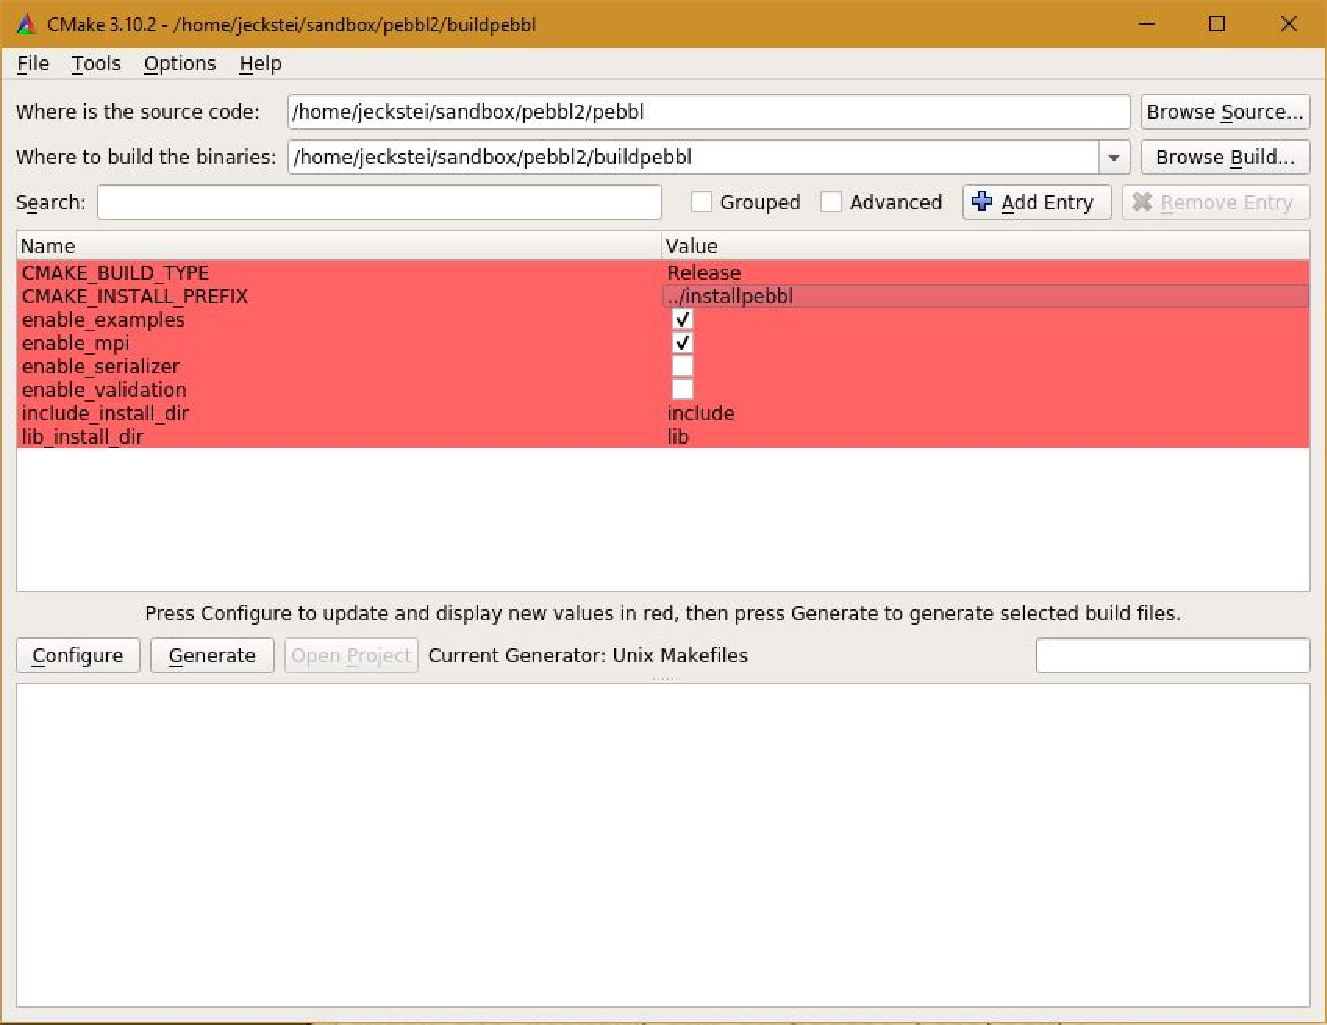
\includegraphics[height=0.45\textheight]{cmake3}
\vspace{-0.3in}
\end{center}{}
\caption{Appearance of \texttt{cmake-gui} after selecting (sample)
configuration options.
  \label{fig:cmake3}}
\end{figure}

Figure~\ref{fig:cmake3} shows the appearance of \texttt{cmake-gui} after
enabling MPI and specifying the directory \texttt{installpebbl} (at the same level as
\texttt{pebbl} and \texttt{buildpebbl}) as the installation target directory.
Press the ``Configure'' button again, and the message pane at the bottom of
the \texttt{cmake-gui} window should the messages shown in
Figure~\ref{fig:cmake4}.  Press the ``Configure'' button once more, and you
should see the messages ``MPI Enabled'' and ``Configuring done'', as shown in
Figure~\ref{fig:cmake5}.  This status indicates that \texttt{cmake} is ready
to generate makefiles.  Press the ``Generate'', after which ``Generating
done'' should appear in the message pane.  At this point, PEBBL has been
configured; you may close the \texttt{cmake-gui} window.

\begin{figure}[tpb]
\begin{center}
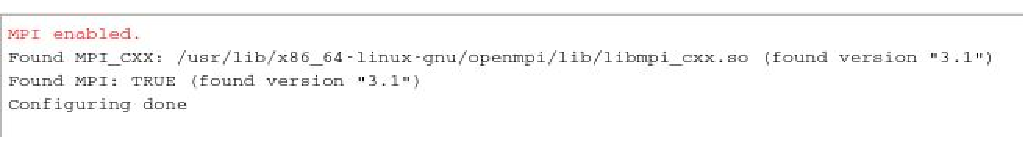
\includegraphics[width=0.8\textwidth]{cmake4}
\vspace{-0.3in}
\end{center}{}
\caption{Appearance of lower \texttt{cmake-gui} pane after second
configuration iteration.
  \label{fig:cmake4}}
\end{figure}

\begin{figure}[tpb]
\begin{center}
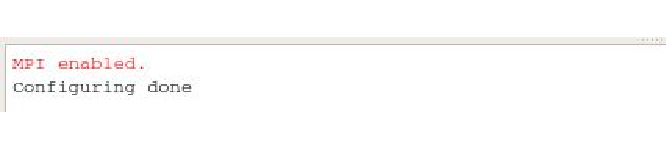
\includegraphics[width=0.5\textwidth]{cmake5.pdf}
\vspace{-0.3in}
\end{center}{}
\caption{Appearance of lower \texttt{cmake-gui} pane after third
configuration iteration (indicating that it is ready generate makefiles).
  \label{fig:cmake5}}
\end{figure}

\subsubsection{Configuring with \texttt{ccmake}}
The \texttt{cmake-gui} configuration process requires an X display.  If an X
display connection is not available or practical, PEBBL may instead by
configured using the \texttt{ccmake} terminal-interface tool or by issuing
\texttt{cmake} shell commands.  This section describes the \texttt{ccmake}
configuration procedure.

You initiate \texttt{ccmake} configuration much as with \texttt{cmake-gui}:
descend into the \texttt{buildpebbl} (or equivalent) directory and enter the
command
\begin{codeblock}
ccmake ../pebbl
\end{codeblock}
Near the top of the terminal screen, you should now see the message
\texttt{EMPTY CACHE}.  Press the \texttt{c} key to initiate the first
\texttt{cmake} configuration cycle.  Shortly, the display should change to
\begin{quote}
\begin{verbatim}
 CMAKE_BUILD_TYPE                *Release
 CMAKE_INSTALL_PREFIX            */usr/local
 enable_examples                 *ON
 enable_mpi                      *OFF
 enable_serializer               *OFF
 enable_validation               *OFF
 include_install_dir             *include
 lib_install_dir                 *lib
\end{verbatim}
\end{quote}
These options have the same interpretation as the those in the previous
section of this document.  You move between options with the keyboard up and
down arrow keys, and pressing the enter key toggles between \texttt{ON} and
\texttt{OFF} settings or allows you to enter new values.  For example, to turn
on debugging, validation, and the parallel layer, while setting the
installation directory to be \texttt{installpebbl} in the same parent
directory as \texttt{buildpebbl}, you would change the options above to
\begin{quote}
\begin{verbatim}
 CMAKE_BUILD_TYPE                *Debug
 CMAKE_INSTALL_PREFIX            *../installpebbl
 enable_examples                 *ON
 enable_mpi                      *ON
 enable_serializer               *OFF
 enable_validation               *ON
 include_install_dir             *include
 lib_install_dir                 *lib
\end{verbatim}
\end{quote}
Press the \texttt{c} key again to initiate another cycle of configuration.
Shortly you shoud see the following display:
\begin{codeblock}
 MPI enabled. \\
\\
Debug mode enabled.
\end{codeblock}
Press the \texttt{e} key to return to the main \texttt{ccmake} display level.
Continue pressing the \texttt{c} and then \texttt{e} keys until the option
\begin{codeblock}
Press [g] to generate and exit
\end{codeblock}
becomes visible among the choices near the bottom of the main \texttt{ccmake}
display screen.  At this point, press the \texttt{g} key; \texttt{ccmake}
should then generate the necessary makefiles and exit.

If you need access to advanced \texttt{cmake} options during the
\texttt{ccmake} configuration process, press the \texttt{t} key to make them
visible.  Pressing \texttt{t} again hides the advanced options.  A few uses
for the advanced options field \texttt{CMAKE\_CXX\_FLAGS} are discussed on
page~\pageref{advancedoptions}.

\subsection{Compiling and installing}
Once the \texttt{cmake} configuration process is complete (using either
\texttt{cmake-gui} or \texttt{ccmake}), you compile PEBBL by simply issuing
the command \texttt{make} in the \texttt{buildpebbl} directory.  The resulting
output should have the following appearance:
{\footnotesize
\begin{verbatim}
Scanning dependencies of target pebbl
[  1%] Building CXX object src/pebbl/CMakeFiles/pebbl.dir/bb/branching.cpp.o
[  2%] Building CXX object src/pebbl/CMakeFiles/pebbl.dir/bb/loadObject.cpp.o
[  3%] Building CXX object src/pebbl/CMakeFiles/pebbl.dir/bb/pebblBase.cpp.o
[  4%] Building CXX object src/pebbl/CMakeFiles/pebbl.dir/bb/pebblParams.cpp.o
[  5%] Building CXX object src/pebbl/CMakeFiles/pebbl.dir/comm/MessageID.cpp.o
[  6%] Building CXX object src/pebbl/CMakeFiles/pebbl.dir/comm/coTree.cpp.o
\end{verbatim}
\vspace{-1.3ex}
$\qquad\vdots$
\begin{verbatim}
[ 96%] Building CXX object src/pebbl/example/CMakeFiles/monomial.dir/monomial.cpp.o
[ 97%] Building CXX object src/pebbl/example/CMakeFiles/monomial.dir/parMonomial.cpp.o
[ 98%] Building CXX object src/pebbl/example/CMakeFiles/monomial.dir/serialMonomial.cpp.o
[100%] Linking CXX executable monomial
[100%] Built target monomial
\end{verbatim}
}

You may accelerate the compilation process by using the \texttt{-j} option of
\texttt{make} to use multiple parallel threads.  For example, on a system with
8 processor cores, you could issue the command
\begin{codeblock}
make -j 8
\end{codeblock}
which would attempt to use 8 processes in parallel to speed up the compilation.

After compilation, the PEBBL object library, \texttt{libpebbl.a} may be found
in the directory \texttt{buildpebbl/src/pebbl}, and the example application
executables (if enabled) may be found in
\texttt{buildpebbl/src/pebbl/example}.

If you wish to use the install procedure, issue the command 
\begin{codeblock}
make install
\end{codeblock}
after the compilation has completed successfully.  If the configured install
directory is a system directory such as \texttt{/usr/local}, you must have
administrator priviledges and use the command \texttt{sudo make install}
instead.

The \texttt{make install} command copies the PEBBL header files and static 
library to the installation directories specified during configuration.  With
the options shown in the previous two subsections, the header and library
files would be copied to \texttt{../installpebbl/include} and
\texttt{../installpebbl/lib}, respectively.

\subsection{Testing}
\label{sec:test}
PEBBL provides a testing script to verify the success of the compilation
process.  In the same \texttt{buildpebbl} directory as you performed the
\texttt{make} operation, you launch the testing script by giving the command
\begin{codeblock}
../pebbl/scripts/testScript.py
\end{codeblock}
The script will only work correctly when run with the current working
directory set to the top of the build directory tree.  The test script does
not require the install step described at the end of the previous section.

If you only configured with the serial layer, the testing script will only
perform serial testing.  In this case, the output should look like:
\begin{quote}
\begin{verbatim}
Only a serial configuration found -- maxprocs reset to 1.
Knapsack tests --
animals.1: 1
animals.2: 1
scor1k.3: 1
test-data.1000.1: 1
Monomial tests --
testdata: 1
pima-indians-diabetes.ss.33.bin: 1
Tests passed
\end{verbatim}
\end{quote}
If you cofigured with the parallel layer, the script defaults to running both
serial tests and parallel tests using between 2 and 32 MPI processes.  In this
situation, its output should look like:
\begin{quote}
\begin{verbatim}
Knapsack tests --
animals.1: 1 2 4 8
animals.2: 1 2 4 8
hard24: 4 8 16 32
scor1k.3: 1 2 4 8 16 32
test-data.1000.1: 1 2 4 8
v24: 4 8 16 32
v24b: 4 8 16 32
Monomial tests --
testdata: 1 2
cmc.data.ss.bin: 16 32
pima-indians-diabetes.ss.33.bin: 1 2 4 8
Tests passed
\end{verbatim}
\end{quote}
For example, \texttt{animals.1:~1 2 4 8} means that the knapsack test instance
\texttt{animals.1} was run successfully in serial and with 2, 4, and 8 MPI
processes (each test instance has a range of MPI process counts in which it
is tested).

The test script has a variety of command-line options, as follows:
\begin{description}
\item[\texttt{--minprocs=}$p$:] The smallest number of MPI processes to be
tested to $p$ (default 1)
\item[\texttt{--maxprocs=}$P$:] The largest number of MPI processes to be
tested to $P$ (default 32 if parallel layer was compiled, and 1 if only the
serial layer wascompiled)
\item[\texttt{--add=}$a$:] The additive step between successive MPI process
counts to be tested (default $0$)
\item[\texttt{--multiply=}$m$:] The multiplicative step between MPI process
counts to be tested (default value $2$)
\item[\texttt{--mpicommand=\emph{command}}:]  The command used to invoke MPI;
the default is \texttt{mpirun}; use \texttt{--mpicommand=mpiexec} on systems
that have \texttt{mpiexec} but not \texttt{mpirun}.
\end{description}
An MPI process count of $1$ denotes using only the serial layer.  The test
script starts at an MPI process count of $p = \mathtt{minprocs}$ and then
updates it by the formula $p \leftarrow mp + a$; thus, the default values of
$m=2$ and $a=0$ cause the processor count to be successivly doubled. You may
also list the options by invoking the script with the single option
\texttt{-h} or \texttt{--help} (in which case no testing is attempted).
